% !TEX root = /Users/vinicius/projects/latex/ee522/main.tex
\documentclass[12pt]{article}
\author{
  Vitor Bergamaschi Dos Santos - 248212\\
  Vinicius De Lima Quadrado - 225357\\
  Leonardo Souza Boaventura - 250417
}
% Pacotes básicos
\usepackage[utf8]{inputenc}
\usepackage[T1]{fontenc}
\usepackage[brazil]{babel}
\usepackage{graphicx}
\usepackage{amsmath, amssymb}
\usepackage{caption}
\usepackage{float}
\usepackage{geometry}
\usepackage{booktabs}
\usepackage{hyperref}
\geometry{a4paper, margin=2.5cm}
\usepackage{indentfirst}
\usepackage{subcaption}
\usepackage[section]{placeins}
\usepackage{float}
\usepackage{pgfplots}
\pgfplotsset{compat=newest}
\usepackage{booktabs}

\usepackage{titlesec}

\setcounter{secnumdepth}{4}

\titleformat{\paragraph}
{\normalfont\normalsize\bfseries}{\theparagraph}{1em}{}
\titlespacing*{\paragraph}
{0pt}{3.25ex plus 1ex minus .2ex}{1.5ex plus .2ex}

\title{\textbf{Relatório de Laboratório -- EE522}}
\date{\textbf{EXPERIMENTO VI:} Microondas
\\ \textbf{Data:} 13/06/2025}

\begin{document}

\maketitle

\section{Objetivos}
Nas seções abaixo seguem os objetivos de cada seção do experimento.

\subsection{Seção I - Demonstração de Propriedades (de Ondas Eletromagnéticas)}
Nesta primeira seção do experimento, um transmissor de microondas
será o foco do estudo, onde serão emitidas ondas polarizadas
linearmente, a uma frequência de 10,525 GHz. Os estudos envolvem a
leitura destas ondas de tensão por meio de um receptor de microondas,
que tem posicionamento controlado por um goniômetro, dessa forma,
busca-se entender o comportamento de eletromagnéticas no espaço e
suas interações com diferentes meios de propagação. Dentro desta
seção será feito experimentos de reflexão, refração, condução em
fibra óptica e polarização de microondas.
\begin{itemize}
  \item Refração: verificaremos a validade da lei da reflexão, que
    postula a igualdade entre ângulos de incidência e reflexão,
    utilizando microondas.
  \item Refração: será determinado experimentalmente o índice de
    refração de um material dielétrico através da lei de Snell.
  \item Fibra óptica: Verificaremos o conceito de ângulo crítico
    aplicado a propagação de microondas em meios confinados.
  \item Polarização: Será analisado os efeitos da polarização em
    microondas, aplicando filtros e verificando como estes afetam a
    transmissão e recepção do sinal.
\end{itemize}

\subsection{Seção II - Cálculo da frequência da fonte}
Nesta seção o objetivo é determinar a frequência da fonte emissora de
microondas, sendo esta uma seção importante para validar a
especificação do equipamento (10,525 GHz) e compreender a relação
entre frequência, comprimento de onda e velocidade de propagação das
ondas eletromagnéticas.
Para tal usaremos dois métodos:
\begin{itemize}
  \item Analisar o padrão de interferência formado por máximos
    consecutivos de intensidade detectados pelo receptor. A distância
    entre máximos será utilizada para calcular o comprimento de onda.

  \item Medir a cavidade metálica de ressonância e analisar os modos
    dominantes de propagação, possibilitando o cálculo da frequência da onda.
\end{itemize}

\subsection{Seção III - Caracterização da antena}
Nesta última seção iremos realizar a caracterização do padrão de
radiação emitidos nos planos de campo elétrico (plano E) e campo
magnético (plano H). Possibilitando visualizar a direcionalidade da
antena, um fator muito importante no projeto de sistemas de
comunicação por ondas eletromagnéticas.

\section{Procedimento Experimental}
Nas seções abaixo seguem os procedimentos experimentais de cada seção
do experimento.

\subsection{Seção I - Demonstração de Propriedades (de Ondas Eletromagnéticas)}
Nesta seção será apresentada a montagem, equipamentos utilizados e
procedimento de execução dos experimentos de reflexão, refração,
condução em fibra óptica e polarização de microondas.

\subsubsection{Reflexão}
Nesta seção será apresentada a montagem, equipamentos utilizados e
procedimento de execução do experimento de reflexão.

\paragraph{Montagem}
O aparato experimental para o estudo da reflexão de microondas foi
montado conforme o diagrama da Figura \ref{fig:img/reflexao.png}, na
figura \ref{fig:img/reflexaomontagem.png} pode-se
verificar a real montagem, com o transmissor e receptor de microondas
dispostos no goniômetro:

\begin{figure}[H]
  \centering
  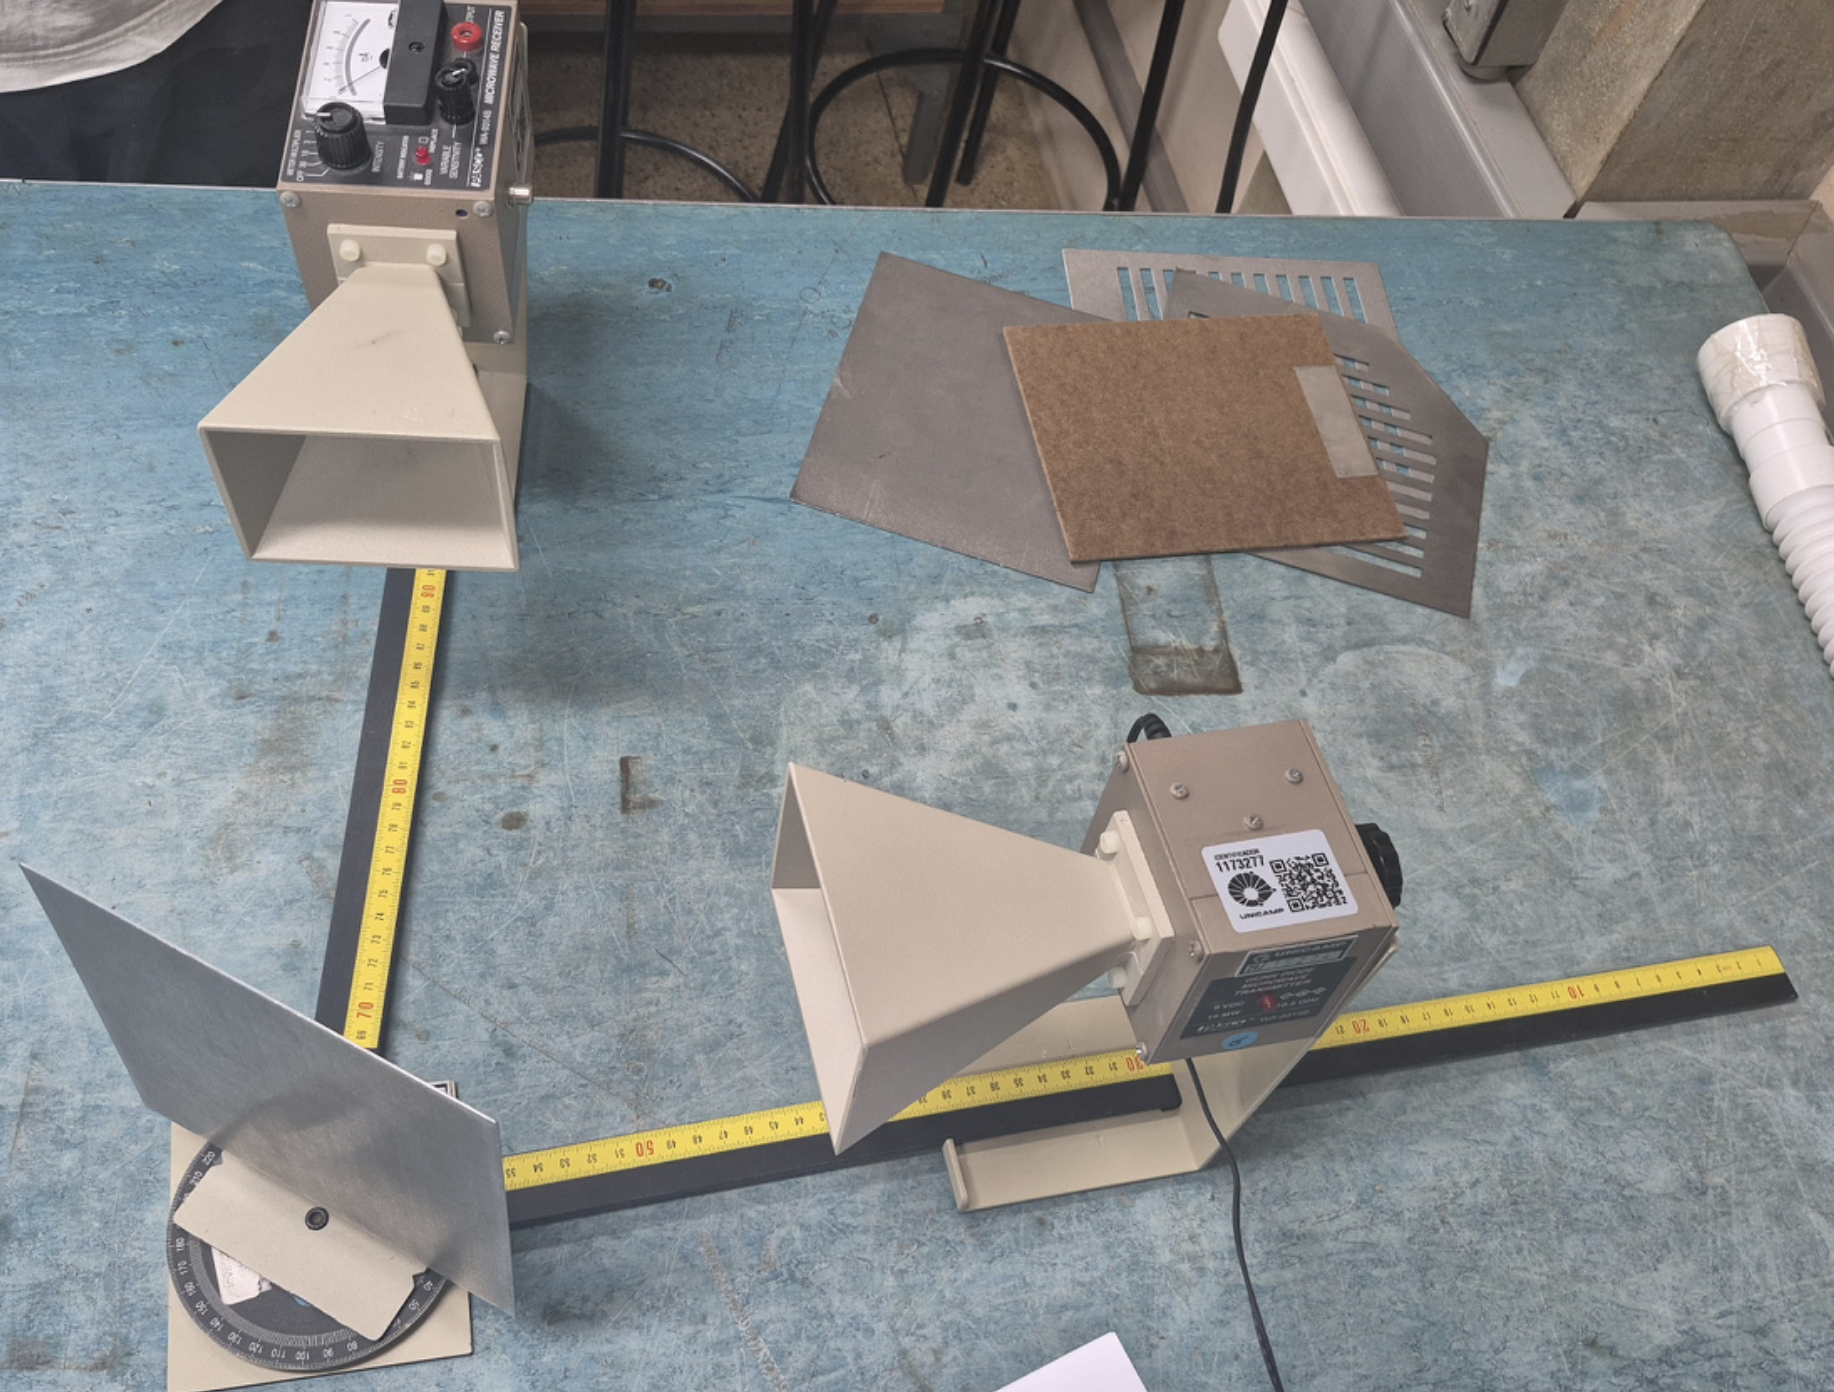
\includegraphics[width=0.8\textwidth]{img/reflexaomontagem.png}
  \caption{Montagem do experimento de reflexão de microondas.}
  \label{fig:img/reflexaomontagem.png}
\end{figure}

\begin{figure}[H]
  \centering
  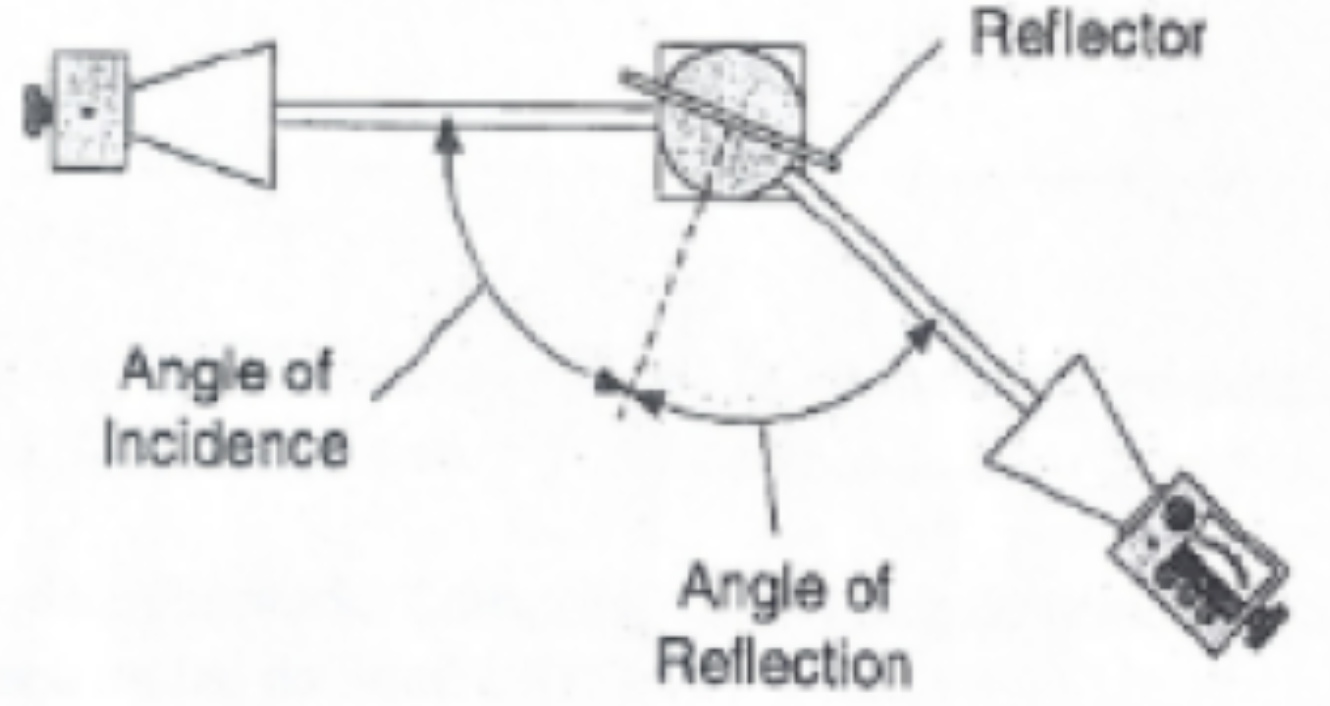
\includegraphics[width=0.8\textwidth]{img/reflexao.png}
  \caption{Ângulo de incidência e reflexão em microondas.}
  \label{fig:img/reflexao.png}
\end{figure}

\paragraph{Equipamentos utilizados}
Foram utilizados um goniômetro, um transmissor de microondas (com
frequência de emissão de 10,525 GHz), um receptor de microondas, um
suporte para anteparo e um anteparo metálico para a reflexão das ondas.

\paragraph{Execução}
A primeira propriedade de ondas eletromagnéticas aferida neste estudo
foi a reflexão. O intuito é aferir o ângulo de reflexão do feixe de
microondas em relação a um determinado ângulo de incidência imposto.
O goniômetro é o elemento crucial para esta medida, visto que permite
manipular o ângulo de posicionamento dos dispositivos com precisão. Na
figura \ref{fig:img/reflexao.png} é possível ver o resultado esperado
em relação ao ângulo de incidência e reflexão, onde o ângulo de
incidência $\theta_i$ é igual ao ângulo de reflexão $\theta_r$.

Na tabela \ref{tab:reflexao} pode-se conferir os resultados mediante 4
medições, ou seja, para cada ângulo de incidência dado, o ângulo de
reflexão é determinado a partir do posicionamento angular do receptor
que confere a leitura do sinal de valor máximo:
\begin{table}[H]
  \centering
  \begin{tabular}{|c|c|}
    \hline
    Ângulo de incidência ($\theta_i$) & Ângulo de reflexão ($\theta_r$) \\
    \hline
    40$^\circ$ & 40$^\circ$ \\
    50$^\circ$ & 50$^\circ$ \\
    60$^\circ$ & 58$^\circ$ \\
    70$^\circ$ & 67$^\circ$ \\
    \hline
  \end{tabular}
  \caption{Resultados da reflexão de microondas.}
  \label{tab:reflexao}
\end{table}

\subsubsection{Refração}
Nesta seção será apresentada a montagem, equipamentos utilizados e
procedimento de execução do experimento de refração.

\paragraph{Montagem}
Para a análise da refração de microondas, ao invés de um anteparo
metálico agora utilizamos um prisma de isopor preenchido com grânulos
de estireno, de forma que se espera o desvio do feixe de ondas em um
determinado ângulo de refração. A figura \ref{fig:img/refracaomontagem.jpeg}
ilustra a montagem do experimento, onde o transmissor e receptor
estão posicionados no goniômetro, com o prisma de isopor entre eles.

Observação: na figura
\ref{fig:img/refracaomontagem.jpeg} o prisma não está
cheio de grânulos de estireno, pois a fotografia foi tirada antes
de completar a montagem, mas o experimento foi realizado com o prisma
preenchido.

\begin{figure}[H]
  \centering
  \includegraphics[width=0.8\textwidth]{img/refracaomontagem.jpeg}
  \caption{Ângulo de incidência e refração em microondas.}
  \label{fig:img/refracaomontagem.jpeg}
\end{figure}

\paragraph{Equipamentos utilizados}
Para esta montagem foram utilizados, além do conjunto transmissor,
goniômetro e receptor, um prisma de isopor preenchido por granulos de
estireno e um suporte para o prisma, como representado na figura
\ref{fig:img/refracaoesquema.png}.

\begin{figure}[H]
  \centering
  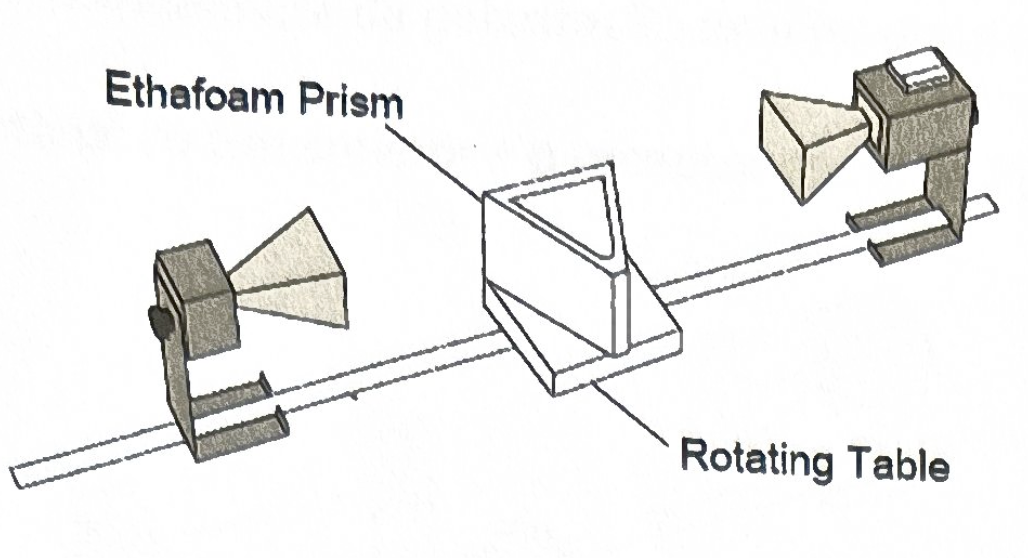
\includegraphics[width=0.8\textwidth]{img/refracaoesquema.png}
  \caption{Esquema da montagem do experimento de refração de microondas.}
  \label{fig:img/refracaoesquema.png}
\end{figure}

\paragraph{Execução}
Assim como no estudo da reflexão, aqui procura-se o ângulo que
confere a máxima leitura de sinal pelo receptor. Rapidamente,
utilizando o goniômetro, é possível aferir o ângulo de refração
$\theta_r = 11^\circ$. A figura \ref{fig:img/refracaografico.png}
abaixo ilustra o ângulo encontrado:

\begin{figure}[H]
  \centering
  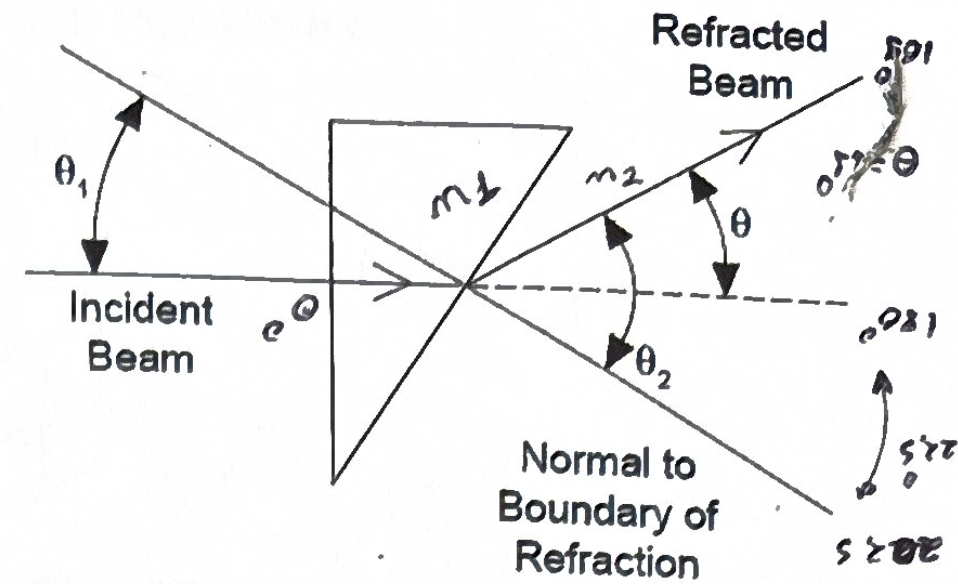
\includegraphics[width=0.8\textwidth]{img/refracaografico.png}
  \caption{Ângulo de incidência e refração em microondas.}
  \label{fig:img/refracaografico.png}
\end{figure}

\subsubsection{Fibra óptica}
Nesta seção será apresentada a montagem, equipamentos utilizados e
procedimento de execução do experimento de fibra óptica. Aqui o
objetivo é verificar a condução das ondas eletromagnéticas por meio
de um tubo preenchido com grânulos de estireno.

\paragraph{Montagem}
A montagem permanece a mesma dos estudos anteriores, com única
diferença que, no lugar do anteparo, há um tubo de plástico dobrável,
preenchido por grânulos de estireno, o qual conecta o transmissor ao
receptor que desta vez estão desalinhados

\paragraph{Equipamentos utilizados}
Para esta montagem foi utilizado o conjunto
transmissor-goniômetro-receptor e um tubo plástico flexível
preenchido com grânulos de estireno que cumpre o papel de fibra
óptica, isto é, um meio condutor de ondas eletromagnéticas.

\paragraph{Execução}
Para aferir a condução das microondas, o transmissor e receptor foram
posicionados a 90º um em relação ao outro, de modo que não haveria
interferência de ondas transmitidas pelo ar. Posicionando o tubo
conectando os dois dispositivos verifica-se sinal lido no receptor,
indicando que o tubo está funcionando como um meio condutor das ondas.

A partir disso, é interessante saber qual o ângulo máximo de flexão
com o qual o tubo permanece conduzindo o feixe de microondas sem
perda significativa de potência do sinal. Para tal, o tubo foi
flexionado em ângulos crescentes, até que o sinal lido pelo receptor
começou a cair significativamente.

\subsubsection{Polarização}
Nesta seção será apresentada a montagem, equipamentos utilizados e
procedimento de execução do experimento de polarização. Será
verificado que ondas eletromagnéticas são transversais, com vetores
do campo elétrico (E) e campo magnético (B) oscilando
perpendicularmente à direção de propagação.

\paragraph{Montagem}
Desta vez utiliza-se um anteparo vazado em formas retangulares
paralelas entre si no eixo do goniômetro, este é o polarizador. Neste
estudo serão utilizados 2 polarizadores alinhados no mesmo eixo, a figura
\ref{fig:img/polarizacao-esquema.png} ilustra o esquema da montagem do
experimento, onde o transmissor e receptor estão posicionados no
goniômetro, com um polarizador entre eles. A figura
\ref{fig:img/polarizacao-onda-polarizada.png} ilustra a onda
atravessando o polarizador, mostrando o resultado esperado de uma onda
polarizada linearmente.

\begin{figure}[H]
  \centering
  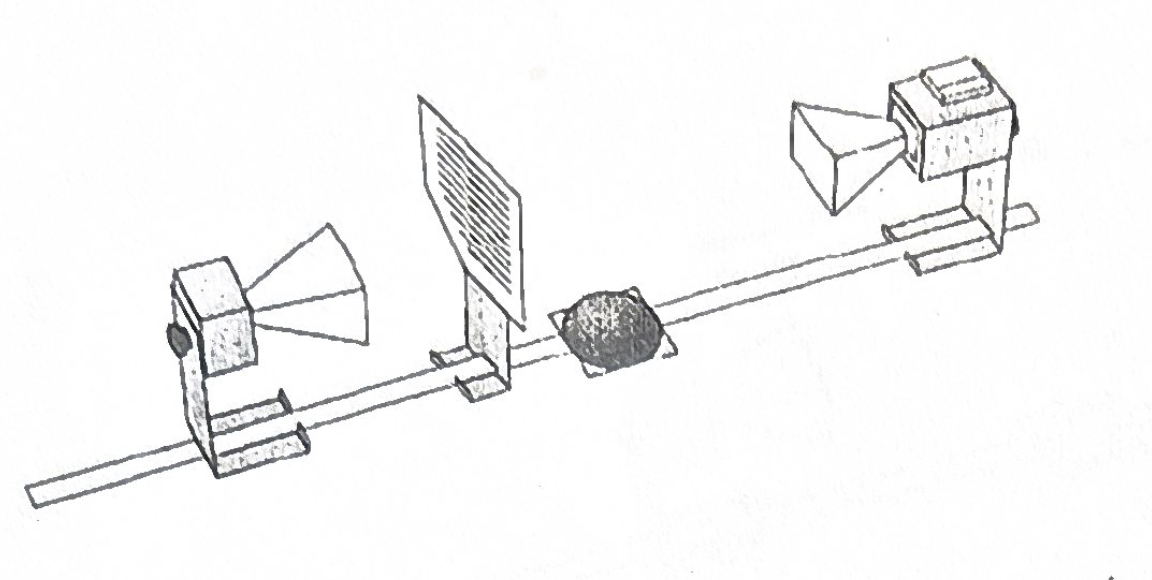
\includegraphics[width=0.8\textwidth]{img/polarizacao-esquema.png}
  \caption{Esquema da montagem do experimento de polarização.}
  \label{fig:img/polarizacao-esquema.png}
\end{figure}

\begin{figure}[H]
  \centering
  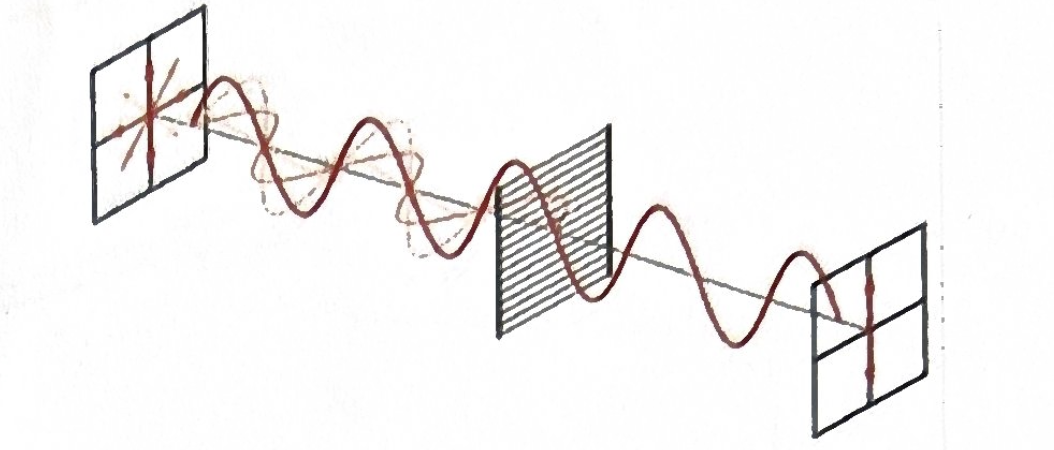
\includegraphics[width=0.8\textwidth]{img/polarizacao-onda-polarizada.png}
  \caption{Onda atravessando o polarizador.}
  \label{fig:img/polarizacao-onda-polarizada.png}
\end{figure}

\paragraph{Equipamentos utilizados}
Além do conjunto transmissor-goniômetro-receptor, foram utilizados os
2 polarizadores metálicos, a figura
\ref{fig:img/polarizacao-filtros.png} ilustra os polarizadores
utilizados, onde é possível ver as aberturas retangulares
paralelas entre si.

\begin{figure}[H]
  \centering
  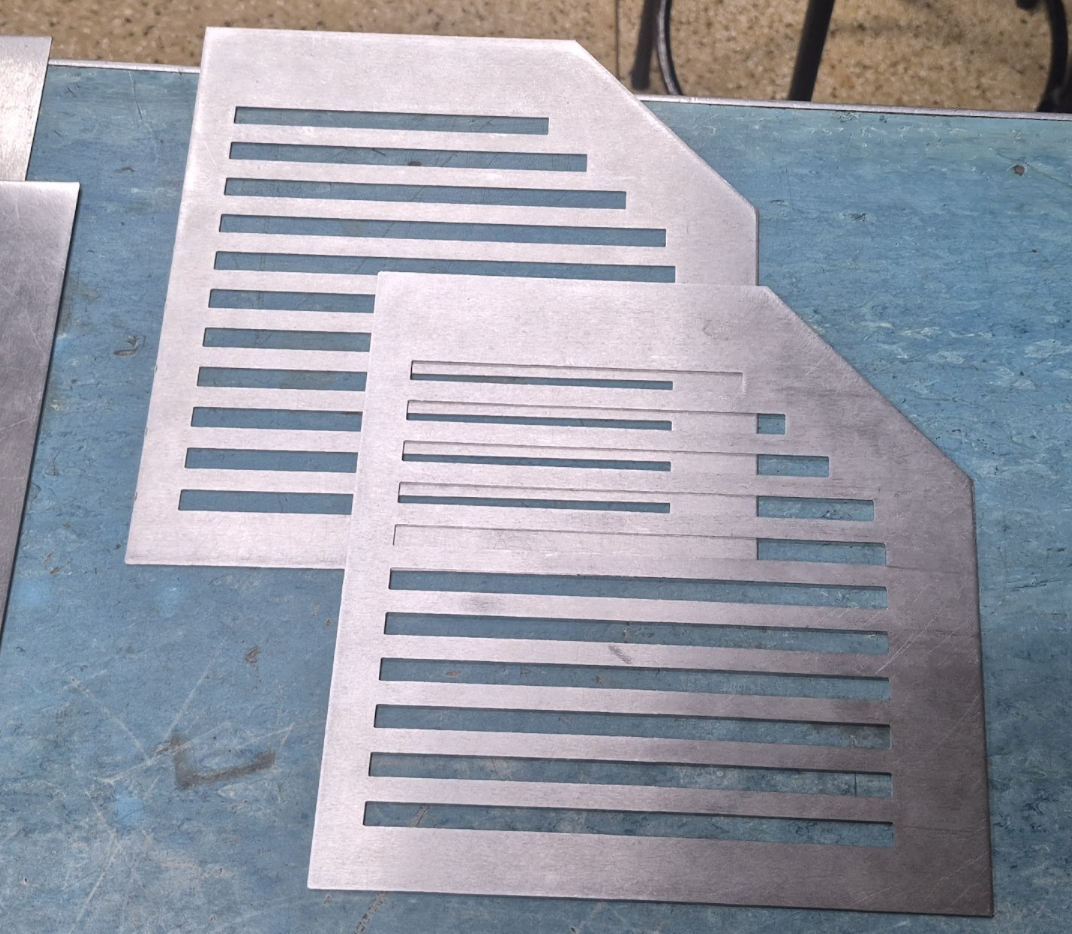
\includegraphics[width=0.8\textwidth]{img/polarizacao-filtros.png}
  \caption{Filtros polarizadores.}
  \label{fig:img/polarizacao-filtros.png}
\end{figure}
\paragraph{Execução}

Iniciamente alinhamos o transmissor e receptor com zero graus de
rotação entre eles, no mesmo eixo de polarização. A partir disso posicionamos
o primeiro polarizador entre eles com suas fendas em zero graus e depois 90
graus, observando a variação do sinal lido pelo receptor. Em seguida o
transmissor e o receptor foram realinhados com 90 graus de rotação entre eles
e o segundo polarizador foi posicionado entre eles com suas fendas orientadas
a 45 graus, registrando novamente a variação do sinal lido pelo receptor.
\subsection{Seção II - Cálculo da frequência da fonte}
Nesta seção será apresentada a montagem, equipamentos utilizados e
procedimento de execução dos experimentos dos método 1 - medição da
distância de máximos de intensidade e método 2 - medição da cavidade
metálica e modos de propagação, ambos métodos para calcular a
frequência da fonte.

\subsubsection{Método 1 - Medição da distância de máximos de intensidade}
Nesta seção será apresentada a montagem, equipamentos utilizados e
procedimento de execução do experimento de medição da distância de
pontos máximos de intensidade de radiação. A figura
\ref{fig:img/metodo1esquema.png}
ilustra o esquema da montagem do experimento.

\begin{figure}[H]
  \centering
  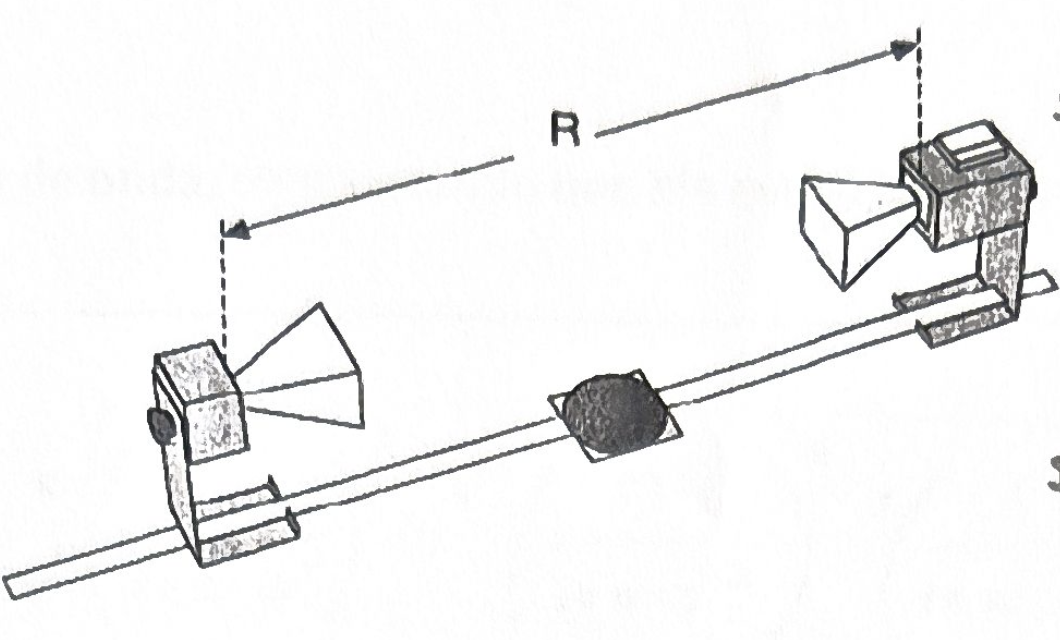
\includegraphics[width=0.8\textwidth]{img/metodo1esquema.png}
  \caption{Esquema da montagem do experimento de medição da distância
  de máximos de intensidade.}
  \label{fig:img/metodo1esquema.png}
\end{figure}

\paragraph{Montagem}
O transmissor e receptor montados sobre o goniômetro,  com
alinhamento de 180 graus entre eles. A figura \ref{fig:img/metodo1montagem.png}
ilustra a montagem do experimento, onde o transmissor e receptor
estão posicionados no goniômetro, com o receptor afastado do
transmissor, de forma que o receptor possa ser afastado
gradativamente até encontrar os máximos de intensidade de radiação.

\begin{figure}[H]
  \centering
  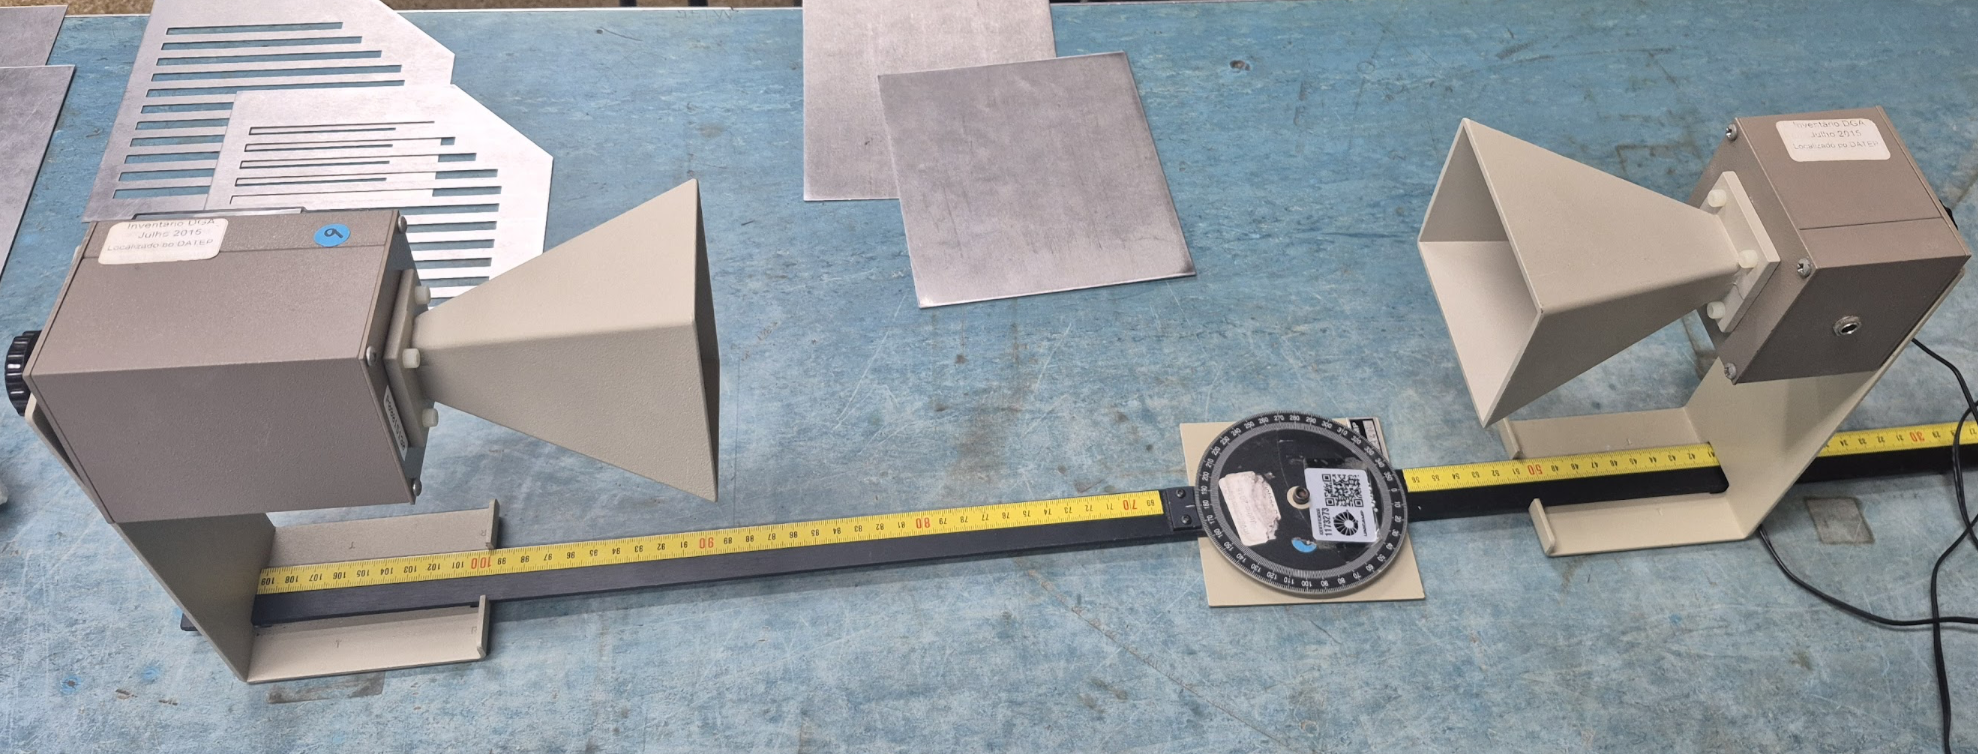
\includegraphics[width=0.8\textwidth]{img/metodo1montagem.png}
  \caption{Montagem do experimento de medição da distância de máximos
  de intensidade.}
  \label{fig:img/metodo1montagem.png}
\end{figure}

\paragraph{Equipamentos utilizados}
Os equipamentos utilizados foram o transmissor, receptor e goniômetro

\paragraph{Execução}
Mantendo sempre o goniômetro medindo 180 graus entre transmissor e
receptor, mantivemos o transmissor parado e afastamos o receptor
gradativamente até encontrar um ponto onde o sinal alcançava o fundo
de escala do receptor.

Tomamos nota da posição do primeiro máximo de intensidade de radiação
encontrada, em seguida afastamos o receptor até encontrar o próximo
máximo. Repetimos isso encontrando os máximos subsequentes até o fim
da escala de distância do goniômetro. A figura
\ref{fig:img/metodo1cavidaderessonante.png}
ilustra a zona de ressonância, onde os máximos de intensidade
são encontrados ao variar a distância do receptor em relação ao
transmissor.

\begin{figure}[H]
  \centering
  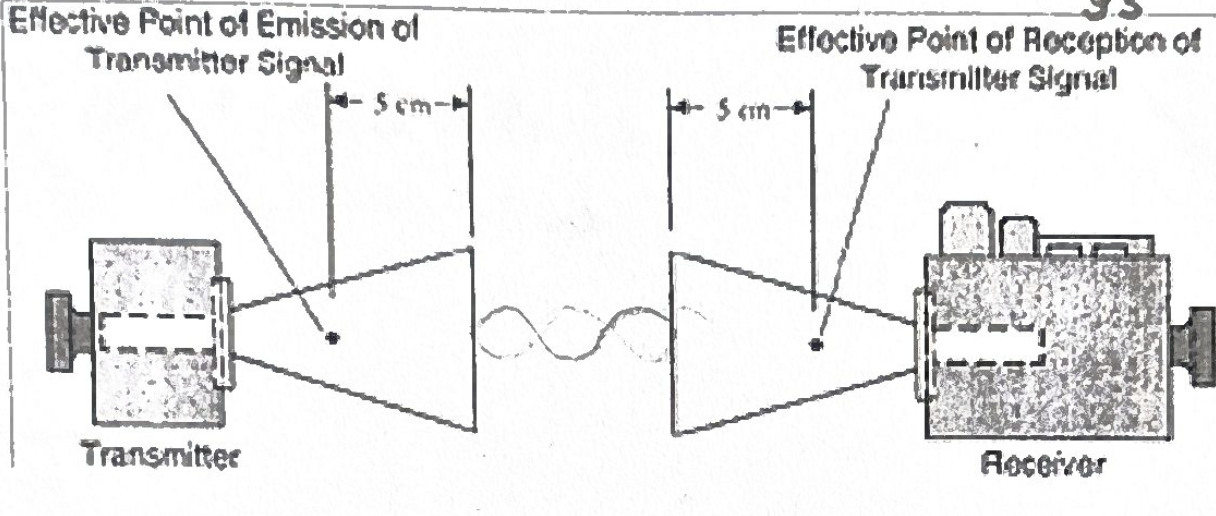
\includegraphics[width=0.8\textwidth]{img/metodo1cavidaderessonante.png}
  \caption{Zona de ressonância.}
  \label{fig:img/metodo1cavidaderessonante.png}
\end{figure}

\subsubsection{Método 2 - medição da cavidade metálica e modos de propagação}
Nesta seção será apresentada a montagem, equipamentos utilizados e
procedimento de execução do experimento de medição da cavidade
metálica e modos de propagação.

\paragraph{Montagem}
O equipamento montado consiste em uma parte interna do emissor
desmontada. Para tal foi retirado 4 parafusos da lateral do emissor
para termos acesso a cavidade ressonante metálica. A figura
\ref{fig:img/metodo2montagem.png} ilustra a montagem do experimento,
onde o transmissor está desmontado e o podemos ver a cavidade metálica
resonante.

\begin{figure}[H]
  \centering
  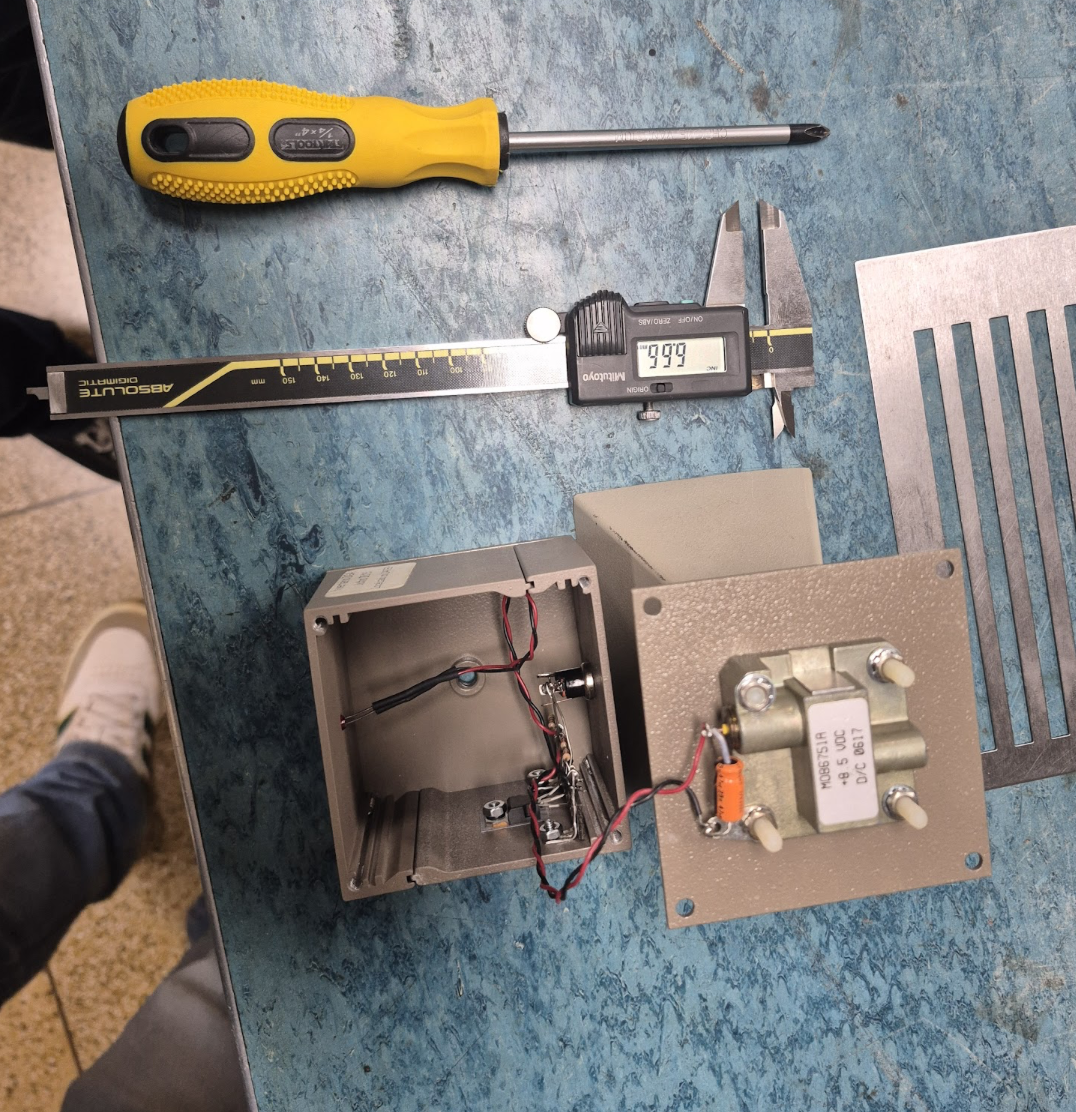
\includegraphics[width=0.8\textwidth]{img/metodo2montagem.png}
  \caption{Montagem do experimento de medição da cavidade metálica e
  modos de propagação.}
  \label{fig:img/metodo2montagem.png}
\end{figure}

\paragraph{Equipamentos utilizados}
Os equipamentos utilizados foram o emissor microondas, chave phillips
e paquímetro.

\paragraph{Execução}
Com o receptor em mãos, foi retirado 4 parafusos laterais do mesmo
com uma chave philips, permitindo acesso a cavidade ressonante
metálica. Esta cavidade teve as dimensões de largura, comprimento e
profundidade medidas com um paquímetro. A figura
\ref{fig:img/metodo2cavidade.png} ilustra a cavidade metálica
ressonante, onde as cotas P, C e L são, respectivamente,
profundidade, comprimento e largura da cavidade.

\begin{figure}[H]
  \centering
  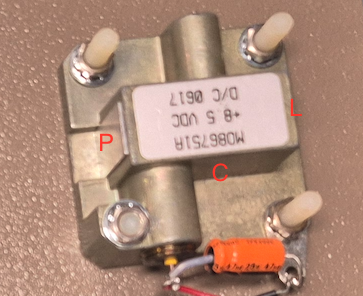
\includegraphics[width=0.8\textwidth]{img/metodo2cavidade.png}
  \caption{Cavidade metálica ressonante. As cotas P, C e L são,
  respectivamente, profundidade, comprimento e largura da cavidade.}
  \label{fig:img/metodo2cavidade.png}
\end{figure}

\subsubsection{Seção III - Caracterização da antena}
Nesta seção será apresentada a montagem, equipamentos utilizados e
procedimento de execução do experimento de caracterização da antena.

\paragraph{Montagem}
Nesta seção serão usadas duas montagens semelhantes, ambas com o
transmissor e receptor montados sobre o goniômetro com ângulo
ajustável e distância fixa. Na primeira montagem onde faremos a
varredura sob o plano E, antena e receptor ficarão alinhados com zero
graus de rotação entre si, já na segunda montagem onde haverá
varredura sobre o plano H os dois ficarão alinhados com 90 graus de
rotação entre si.

\paragraph{Equipamentos utilizados}
Os equipamentos utilizados serão receptor, emissor e goniômetro.

\paragraph{Execução}
Mantendo receptor e emissor fixos na escala de distância entre eles e
movendo apenas de modo angular, iniciamos uma varredura no plano E,
com receptor e emissor alinhados com zero graus de rotação entre
eles. O ponto de partida se dá na escala de zero graus do goniômetro,
ajustamos a escala do receptor para receber a máxima intensidade
neste ponto (fundo de escala) e iniciamos a varredura do plano E
movimentando 90 graus para a direita, retomando ao ponto de zero
graus, e por fim movimentando 90 graus para a esquerda. Ambas as
varreduras foram feitas com incrementos de 5 graus.

Para realizar a varredura no plano H o receptor foi rotacionado 90
graus em relação ao emissor e o processo descrito acima foi realizado novamente.

\section{Resultados}
Nos capítulos abaixo seguem as discussões dos resultados de cada
seção do experimento.

\subsection{Seção I - Demonstração de Propriedades (de Ondas Eletromagnéticas)}
\subsubsection{Reflexão}
\paragraph{Apresentação de dados}
\paragraph{Análise dos resultados}

\subsubsection{Refração}
\paragraph{Apresentação de dados}
\paragraph{Análise dos resultados}

\subsubsection{Fibra óptica}
\paragraph{Apresentação de dados}
\paragraph{Análise dos resultados}

\subsubsection{Polarização}
\paragraph{Apresentação de dados}
\paragraph{Análise dos resultados}

\subsection{Seção II - Cálculo de Frequência de Fonte}
\subsubsection{Método 1 - Medição da distância de máximos de intensidade}
\paragraph{Apresentação de dados}
\paragraph{Análise dos resultados}

\subsubsection{Método 2 - Medição da cavidade metálica e modos de propagação}
\paragraph{Apresentação de dados}
\paragraph{Análise dos resultados}

\subsection{Seção III - Caracterização da antena}
\subsubsection{Apresentação de dados}
\subsubsection{Análise dos resultados}

\clearpage
\section{Conclusão}

\clearpage
\begin{thebibliography}{9}
  \bibitem{ref1}
  KRAUS, J.D. Eletromagnetics. 4th ed. McGraw-Hill, 1991.

  \bibitem{ref2}
  REITZ, J.R., MILFORD, F.J. \& CHRISTY, R.W. Foundations of
  Electromagnetic Theory. 3rd Addison-Wesley, 1980.

  \bibitem{ref3}
  Feynman, R.P., Leighton, R.B., Sand, M. The Feynman Lectures on
  Physics, Volume II – mainly electromagnetism and matter. Disponível
  em: \url{https://www.feynmanlectures.caltech.edu/II_toc.html}.
  Acesso em: 13 jun. 2025.
\end{thebibliography}
\end{document}
